\documentclass{article}
\usepackage{tikz}
\usetikzlibrary{angles, quotes}
\usepackage{amssymb}
\usepackage{pgfplots}
\pgfplotsset{width=10cm,compat=1.9}
\usepgfplotslibrary{statistics}
\usepackage[left=2.54cm,right=2.54cm,top=2.54cm,bottom=2.54cm]{geometry}
\usepackage{tasks} %Paquete necesario para la producción de items horizontales para algunos ejercicios de tarea empleando el comando /begin{multicols}}{#}.../end{multicols} para ayudarnos a reducir las páginas
\usepackage{pdflscape} %comando que permite cambiar a orientación horizontal las hojas%
\usepackage{soul} %Paquete para permitir la compilación de acentos usando el comando {\hl{}}}\\
\sethlcolor{yellow(munsell)} %comando para definir el color para el subrayado usando el comando \hl
\usepackage[utf8]{inputenc}
\usepackage[spanish]{babel}
\usepackage{icomma}
\usepackage{ragged2e}
\usepackage{siunitx}
\usepackage{url}
\usepackage[colorlinks=true, urlcolor=blue,  linkcolor=black, citecolor=green]{hyperref}
\usepackage{pdfpages}
\usepackage{blindtext} %Paquete que genera texto ficticio (dummy text) con el comando: \blindtext
\usepackage{cancel} %in the preamble gives you four different modes of striking through: \cancel{text to cancel} draws a diagonal line (slash) through its argument, \bcancel{text to cancel} uses the negative slope (a backslash), \xcancel{text to cancel} draws an X (actually \cancel plus \bcancel), \cancelto{〈value〉}{〈expression〉} draws a diagonal arrow through the 〈expression〉pointing to the 〈value〉 (math-mode only)
\usepackage{csquotes}
\usepackage{afterpage}
\usepackage{parskip} 
\usepackage{float}
\usepackage{enumitem}
\usepackage{multicol}%Paquete que permite la creación aislada de columnas de texto. De esta forma se reduce la cantidad de páginas en nuestro documento
\usepackage{lipsum} %Paquete que genera texto de relleno al igual que \usepackage{blindtext}, se usa con el comando \lipsum[#-#] los #(hashtags) delimitan el número de páginas que deseamos ocupar del paquete lipsum para usarlos como relleno. 

% Definir el comando personalizado para la nota
\newcommand{\mynote}[1]{%
\begin{tikzpicture}[baseline=-0.75ex]
	\node[draw, circle, fill=Apple Green!60, inner sep=2pt] (note) {\textbf{Nota:}};
\end{tikzpicture}%
\ \textit{#1}%
}

\newenvironment{Figura}
{\par\medskip\noindent\minipage{\linewidth}}
{\endminipage\par\medskip}
\usepackage{caption}
\usepackage[
backend=biber,
sorting=none,
url=true
]{biblatex} %bibliografía
\addbibresource{biblio.bib}
% Establecer el espacio entre las entradas de la bibliografía
\setlength{\bibitemsep}{1\baselineskip} % Puedes ajustar el valor según tus preferencias
\usepackage{amsmath,amsthm,amssymb,amsfonts}
\usepackage{pifont} %Permite la compilación del comando \xmark: es el símbolo de la tachita
\usepackage{mathtools} %permite la compilación de símbolos para matrices
\usepackage{empheq} %Paquete que se relaciona con \usepackage[most]{tcolorbox} para la creación de cuadros/cajas de colores para delimitar los resultados matemáticos o líneas de texto usando la línea de comando: \begin{empheq}[box={\mymath[colback=orange(webcolor)!70,drop lifted shadow]}]{equation*} \end{empheq}
\usepackage[most]{tcolorbox} %Paquete que se relaciona con \usepackage{empheq} para la creación de cuadros/cajas de colores para delimitar los resultados matemáticos o líneas de texto
\renewcommand{\qedsymbol}{$\blacksquare$}
\usetikzlibrary{positioning,decorations.pathreplacing} %Paquete que permite la compilación de llaves para cuadros sinópticos (brace diagram) 
\usepackage{schemata} %The schemata package is designed just for these brace diagrams
\usepackage{booktabs}

\newcommand\AB[2]{\schema{\schemabox{#1}}{\schemabox{#2}}} %comando o paquete necesario para crear cuadros sinópticos

\newtcbox{\mymath}[1][]{%
nobeforeafter, math upper, tcbox raise base,
enhanced, colframe=blue!30!black,
colback=blue!30, boxrule=1pt,
#1} %Comando importante para encasillar los resultados matemáticos en cajas de diferentes colores, se relaciona con los paquetes \usepackage{empheq} y \usepackage[most]{tcolorbox} 

\newenvironment{sysmatrix}[1]
{\left(\begin{array}{@{}#1@{}}}
{\end{array}\right)}
\newcommand{\ro}[1]{%
\xrightarrow{\mathmakebox[\rowidth]{#1}}%
}
\newlength{\rowidth}% row operation width
\AtBeginDocument{\setlength{\rowidth}{3em}}  %Comando importante para laproducción de lineas de operaciones entre matrices, método de Gauss o Gauss Jordan se relaciona con \newenvironment{sysmatrix}

%formato para cambiar el horario a español
\usepackage[spanish]{datetime2}
\DTMsetdatestyle{spanish}

\renewcommand{\today}{\DTMdisplaydate{\the\year}{\the\month}{\the\day }{-1}}
%%%%%%%%%%%%%%%%%%%%%%%%%%%%%%%%%%%%%%%%%

\usepackage{datetime}
\newcommand{\mycurrenttime}{\xxivtime}

%%%%%%%%%%%%%%%%%%%%%%%%%%%%%%%%%%%%%%%%%%%%%%%%%%%%%%%%%%%%%%%%%%%%%%%%%%%%%%%%%%%%%%%%%%%%%%%%%%%%%%%%%%%%%%%%%%%%%%%%%%%%%%%%%%%%%%%%%%%%%%%%%


%%%%%%%%%%%%%Caja de color para el título%%%%%%%%%%%%%%%%%%%%%%%%%%%%%%%%%%%%%%%%%%%%%%%%%%%%%%

\definecolor{myframecolor}{RGB}{1, 45, 75} % Prussian Blue
\definecolor{myboxcolor}{RGB}{0, 107, 92} % Apple Green

\newtcolorbox{mybox}{
enhanced,
colback=myboxcolor!7, % Color de fondo del cuadro
colframe=myframecolor, % Color del marco del cuadro
arc=0pt,
boxrule=1pt,
borderline west={2mm}{-10mm}{myframecolor}, % Borde en el lado izquierdo
sharp corners=southwest,
width=\linewidth,
before=\par\vspace{\bigskipamount}, % Espacio antes del cuadro
after=\par\vspace{\bigskipamount} % Espacio después del cuadro
}


\newcommand{\euler}{e} %Comando para producir letra e de euler
\newenvironment{remark}{\par\vfill\footnotesize % Vertical white space above the remark and smaller font size
\begin{list}{}{
		\leftmargin=80pt % Indentation on the left
		\rightmargin=60pt}\item\ignorespaces % Indentation on the right
	\makebox[-2.5pt]{\begin{tikzpicture}[overlay]
			\node[draw=Horizon!60,line width=2.5pt,circle,fill=Horizon!25,font=\sffamily\bfseries,inner sep=4pt,outer sep=0pt] at (-19pt,5pt){\textcolor{Horizon}{Nota}};\end{tikzpicture}} % Blue Nota in a circle
	\advance\baselineskip -1pt}{\end{list}\vskip5pt} % Tighter line spacing and white space after remark
	\usepackage{graphicx}
	
	\usepackage{titling}
	
	\input{colores.tex}
	
	%%Producir signos de cita textual``Asignatura''
	
	\newcommand{\xmark}{\ding{55}} %%%comando que genera la tachita
	
	\newenvironment{MyColorPar}[1]{%
\leavevmode\color{#1}\ignorespaces%
}{%
}%

%%%%%%%%%%%%%%%%%%% Título de la tarea, Nombre de alumno

\title{ \textcolor{Tarawera}{\textbf{T-\textcolor{Sun}{\textbf{2}}}}: \textcolor{Apple Green}{\textbf{\textcolor{orange(colorwheel)}{\textbf{Planilandia}}: una novela de muchas dimensiones}}}
\author{\emph{Julio Alfredo Ballinas García} $\boldsymbol{\mid}$ 202107583}
\date{\today}

%%%%%%%%%%%%%%%%%%% Datos de la Materia

\usepackage{fancyhdr}
\fancypagestyle{plain}{%  the preset of fancyhdr 
\fancyhf{} % clear all header and footer fields
\fancyfoot[R]{
\includegraphics[width=2cm]{LogoFCFMBUAP (1).png}}
\fancyfoot[L]{{\bfseries{\thedate{}}} a las {\bfseries{\mycurrenttime{}}} horas{} (GMT-6, H. Puebla de Zaragoza, Pue)}
\fancyhead[L]{Enseñanza de la física }
\fancyhead[R]{\theauthor}
}
\makeatletter
\def\@maketitle{%
\newpage
\null
\vskip 1em%
\begin{center}%
	\let \footnote \thanks
	{\LARGE \@title \par}%
	\vskip 1em%
	%{\large \@date}%
\end{center}%
\par
\vskip 1em}
\makeatother

\usepackage{lipsum}  
\usepackage{cmbright}


%%%%%%%%%%%%%%%%%%%%%%%%%%%%%%%%%%%%%%%%%%%%%%%%%%%%%%%%%%%%%%%%%%%%%%%%%%%%%%%%%%%%%%%%%%%%%%%%%%%%%%%%%%%%%%%%%%%%%%%%%%%%%%%%%%%%%%%%%%%%%%%%%%%%%%%%%%%%%%%%%%%%%%%%%%%%%%%%%%%%%%%%%%%%%%%%%%%%%%

\begin{document}



\maketitle


%%%%%%%%%%%%%%%%%%% Datos del profesor, campus y aula

\begin{mybox}
	\noindent\begin{tabular}{@{}ll}
		{\bfseries{Profesor}} & Dr. Apolonio Juárez Nuñez\\
		\textcolor{prussianblue}{\bfseries{Campus}} / \textcolor{trueblue}{\bfseries{Facultad}}  & \textcolor{prussianblue}{\bfseries{C.U. BUAP}} /  \textcolor{trueblue}{\bfseries{FCFM}} \\
		\textcolor{prussianblue}{\bfseries{Edificio}} /  \textcolor{trueblue}{\bfseries{Salón}}    & 	\textcolor{prussianblue}{\bfseries{1FM4}} /  \textcolor{trueblue}{\bfseries{104}}   
	\end{tabular} 
\end{mybox} \vspace{1cm}

\section*{Instrucciones de la actividad}
\addcontentsline{toc}{section}{Instrucciones de los ejercicios}

\setlength{\columnsep}{2cm}
\begin{multicols}{2} % Comienza las dos columnas
	%Comienza el primer entorno enumerate
	\begin{enumerate}[label={{\textcolor{trueblue}{\textbf{Ej}. \arabic*.0}}}, start=1]
	\item Para esta actividad se deberán realizar \emph{resúmenes} que cubran los capítulos \textbf{13 al 22} del libro titulado 
\textcolor{orange(colorwheel)}{\textbf{Planilandia}}: 
\textcolor{Apple Green}{\textbf{una novela de muchas dimensiones}}, del autor \textbf{Edwin Abbott Abbott} 
(o \textbf{\emph{Flatland}: \emph{A Romance of Many Dimensions}} en su versión original en inglés).  
Cada resumen deberá incluir, al final, su respectiva \underline{\textbf{opinión personal}}.
	\end{enumerate}
\end{multicols} 

\vspace{2cm}


\tableofcontents  \vspace{2cm}

\section*{\textcolor{Tarawera}{Capítulo 13: \emph{Cómo tuve una visión de Linealandia}}}
\addcontentsline{toc}{section}{Capítulo 13: Cómo tuve una visión de Linealandia}

\subsection*{Resumen}
\addcontentsline{toc}{subsection}{Resumen}

En este capítulo se describe que \textbf{Cuadrado} tiene un \textbf{extraño sueño} en el que logra observar un mundo completamente distinto al suyo, al que se le llama 
\textcolor{Apple Green}{\textbf{Linealandia}}. Puede ver ante sí una gran cantidad de \underline{pequeñas líneas y puntos luminosos} que se mueven de un lado a otro sobre una misma línea. Todo ocurre de manera ordenada, pero para él resulta muy confuso, ya que está acostumbrado a un mundo con más direcciones y más movimiento.

Podemos notar que en Linealandia \textbf{todo ocurre en una sola línea}. Sus habitantes solo pueden avanzar hacia adelante o hacia atrás, pero jamás pueden subir, bajar o rodear a alguien. \textbf{Cuadrado} intenta hablar con uno de esos seres, creyendo que se trata de una mujer, pero aquel ser le responde que en realidad es el 
\underline{\textbf{Rey de Linealandia}}. Desde ese momento empieza una conversación muy curiosa entre ambos.

El rey está completamente convencido de que su línea es \emph{todo el universo} y que fuera de ella no existe absolutamente nada. Para él, pensar en otros mundos o espacios es algo imposible. Incluso cuando escucha la voz de \textbf{Cuadrado}, no puede entender de dónde viene, pues no logra verlo como una figura completa, sino solo como sonidos que aparecen dentro de su línea.

Como se puede observar en la 
\textcolor{Lochmara}{\textbf{Figura \ref{fig:linealandia}}}, 
la visión del mundo en Linealandia es completamente limitada a una sola línea, donde los habitantes solo pueden percibir puntos que aparecen y desaparecen conforme se acercan o se alejan.

\begin{figure}[H]
    \centering
    \fcolorbox{Tarawera}{Cinnabar}{
        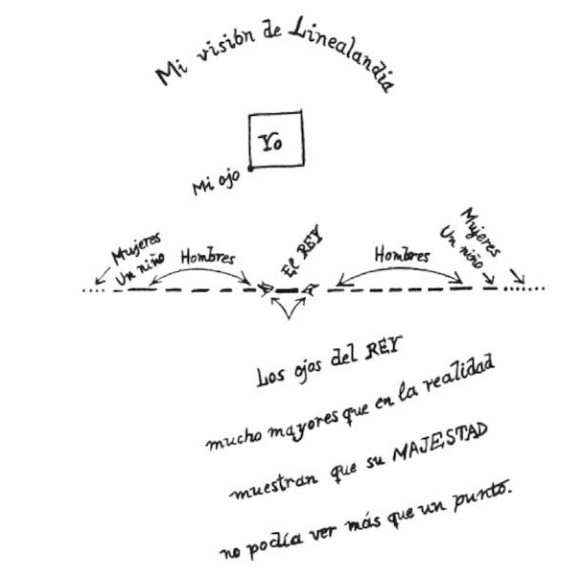
\includegraphics[width=0.6\textwidth]{linealandia.png}
    }
    \caption{\textcolor{Tarawera}{\textbf{Representación de la visión de Cuadrado en Linealandia.}}}
    \label{fig:linealandia}
\end{figure}

Se nos cuenta también cómo viven los habitantes de este lugar. Nadie puede rebasar a otro, por lo que los vecinos están condenados a ser vecinos \textbf{para siempre}. No existe forma de rodear a alguien ni de cambiar de lugar con facilidad. Todo está limitado a un solo camino recto. \textbf{Cuadrado} considera que esta forma de vida es \underline{monótona y repetitiva}, pero le sorprende que el rey se muestre alegre y orgulloso de su mundo.

Con curiosidad, \textbf{Cuadrado} le pregunta al rey por su familia. El rey responde que tiene \textbf{dos esposas} e hijos, lo cual lo desconcierta todavía más. Entonces el rey explica que en Linealandia las uniones no se hacen por cercanía física, sino por medio de las \emph{voces y los sonidos}. Cada cierto tiempo, los habitantes participan en una especie de 
\textcolor{Cerulean}{\textbf{coro universal}}, donde buscan armonizar sus voces hasta formar una unión.

Cuando las voces coinciden de forma correcta, se forma una familia y nacen nuevos habitantes. Así es como se organiza la vida en Linealandia. \textbf{Cuadrado} queda sorprendido por esta forma tan extraña de relación, tan distinta a todo lo que él conoce. A pesar de ello, el rey sigue convencido de que su mundo es el único que existe y que pensar en algo diferente es una completa locura.

A lo largo del capítulo se puede notar que el rey no acepta ninguna idea que contradiga su forma de ver la realidad. Para él, fuera de su línea \underline{no hay nada}. De esta manera, el capítulo nos muestra un mundo limitado en espacio, pero también en \textbf{forma de pensar}.

\subsection*{Opinión personal}
\addcontentsline{toc}{subsection}{Opinión personal}

En lo personal, este capítulo me pareció \textbf{muy interesante y creativo}, porque nos hace reflexionar sobre cómo muchas veces las personas están completamente seguras de que su forma de ver el mundo es la única correcta. El rey de Linealandia está tan convencido de su realidad que \underline{ni siquiera se permite dudar} de que exista algo más allá de su línea.

Me llamó mucho la atención que los habitantes de Linealandia vivan con tantas limitaciones y aun así se sientan completamente satisfechos. Creo que esto nos enseña que las personas pueden acostumbrarse a casi cualquier situación cuando \emph{no conocen otra realidad}. Para ellos, su mundo es normal y no sienten la necesidad de buscar algo distinto.

También me pareció curioso que el matrimonio se forme por medio de las voces y no por la cercanía entre las personas. Esto muestra que cada sociedad construye sus propias reglas de acuerdo con su forma de existir. Aunque desde nuestro punto de vista puede parecer extraño, dentro de su mundo tiene todo el sentido.

Por otro lado, considero que el rey representa a muchas personas que se \textbf{cierran completamente a nuevas ideas}. Aunque \textbf{Cuadrado} intenta mostrarle que puede existir algo más, el rey se burla de esa posibilidad. Esto me hizo pensar que no siempre es fácil aceptar lo desconocido y que, muchas veces, preferimos quedarnos con lo que ya entendemos, aunque sea limitado.


\section*{\textcolor{Apple Green}{Capítulo 14: \emph{Cómo intenté en vano explicar la naturaleza de Planilandia}}}
\addcontentsline{toc}{section}{Capítulo 14: Cómo intenté en vano explicar la naturaleza de Planilandia}

\subsection*{Resumen}
\addcontentsline{toc}{subsection}{Resumen}

En este capítulo se describe cómo \textbf{Cuadrado} intenta, con mucha paciencia, explicarle al \underline{\textbf{Rey de Linealandia}} cómo es realmente el mundo de Planilandia. \textbf{Cuadrado} trata de hacerle ver que en su mundo no todo es una sola línea, sino que existen \emph{figuras con ancho} y que hay más direcciones además de avanzar hacia adelante o hacia atrás.

El rey, sin embargo, se muestra desde el principio \underline{muy cerrado a estas ideas}. Para él, solo existe lo que puede oír, pues en Linealandia el sentido más importante es el \textbf{oído}. El rey asegura que, por medio de las voces, puede conocer la forma, el tamaño y la posición de todos sus súbditos, incluso la de sus esposas. Por eso considera que el sentido de la vista no es necesario.

\textbf{Cuadrado} intenta hacerle ver la diferencia entre un punto y una línea usando ejemplos, pero el rey se burla de esas explicaciones. Para él, decir que existe algo como “derecha” e “izquierda” fuera de su línea no tiene ningún sentido. Incluso cuando \textbf{Cuadrado} habla de moverse en distintas direcciones, el rey no puede imaginarlo.

Como se puede observar en la 
\textcolor{Lochmara}{\textbf{Figura \ref{fig:salida-linea}}}, 
\textbf{Cuadrado} intenta demostrar lo que dice saliendo poco a poco de la propia línea de Linealandia, algo que para el rey resulta completamente imposible de concebir.

\begin{figure}[H]
    \centering
    \fcolorbox{Apple Green}{Gallery}{
        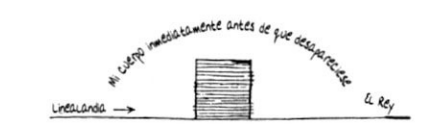
\includegraphics[width=0.6\textwidth]{salida.png}
    }
    \caption{\textcolor{Apple Green}{\textbf{Cuadrado saliendo de la línea de Linealandia para demostrar otra forma de espacio.}}}
    \label{fig:salida-linea}
\end{figure}

Cuando \textbf{Cuadrado} logra salir por completo de la línea, el rey entra en pánico, pues cree que ha desaparecido o que ha muerto. Pero en realidad, \textbf{Cuadrado} ahora puede ver la línea desde afuera y observar al mismo tiempo a los habitantes que están al norte y al sur de ella, algo que en Linealandia es imposible de hacer.

A pesar de esta demostración, el rey se niega a aceptar lo que está ocurriendo. Piensa que todo se trata de trucos y engaños. Incluso llega a enfurecerse cuando \textbf{Cuadrado} afirma que él mismo es un cuadrado y no una simple línea. El rechazo del rey crece tanto que termina provocando un gran alboroto entre sus súbditos.

Justo en el momento de mayor tensión, cuando parece que todo terminará mal para \textbf{Cuadrado}, el sueño se rompe y él \emph{despierta} de golpe en su propio mundo. Así termina su intento fallido de hacer comprender al rey que existe una realidad mucho más amplia que la que él conoce.

\subsection*{Opinión personal}
\addcontentsline{toc}{subsection}{Opinión personal}

En lo personal, este capítulo me pareció \textbf{muy frustrante, pero muy real}. \textbf{Cuadrado} hace todo lo posible por explicarle al rey que existe algo más allá de su mundo, incluso se arriesga a demostrarlo con hechos, pero aun así el rey \underline{se niega a creer}. Esto me hizo pensar en lo difícil que es cambiar la forma de pensar de alguien que está completamente convencido de tener la verdad.

Me llamó mucho la atención cómo el rey confía ciegamente en el oído y desprecia por completo la vista. Esto muestra que cuando una persona está acostumbrada a una sola forma de conocer el mundo, puede llegar a pensar que esa es la \emph{única válida}. Todo lo que queda fuera de su experiencia lo considera imposible.

También me pareció muy fuerte el momento en que el rey se enfurece y comienza a llamar a \textbf{Cuadrado} un mentiroso y un monstruo solo por pensar distinto. Esto refleja cómo el miedo a lo desconocido puede transformarse fácilmente en rechazo y violencia.

Este capítulo me deja una enseñanza muy clara: \underline{no siempre la verdad es aceptada aunque esté frente a los ojos}. Muchas veces las personas prefieren quedarse con lo que ya conocen, aunque sea limitado, antes que abrirse a nuevas ideas.

\section*{\textcolor{Cerulean}{Capítulo 15: \emph{Sobre un desconocido de Espaciolandia}}}
\addcontentsline{toc}{section}{Capítulo 15: Sobre un desconocido de Espaciolandia}

\subsection*{Resumen}
\addcontentsline{toc}{subsection}{Resumen}

En este capítulo se pasa de los sueños a los hechos. \textbf{Cuadrado} está tranquilamente en su casa con su esposa, reflexionando sobre el cambio de siglo y recordando una conversación con su nieto, un pequeño hexágono muy inteligente. El niño le pregunta por el significado de elevar un número al cubo, es decir, qué puede representar un número como \(9^3\) en geometría. \textbf{Cuadrado}, muy seguro de sí mismo, responde que \underline{eso no significa nada}, pues en Planilandia solo existen dos dimensiones.

Después de esto, \textbf{Cuadrado} comienza a sentir una \textbf{extraña presencia} en la habitación. Aunque mira a su alrededor, no ve nada, pero siente claramente que \emph{alguien más está ahí}. En ese momento escucha una voz que contradice lo que acaba de decir: le asegura que el niño no es tonto y que \(9^3\) \underline{sí tiene un significado}.

De pronto, aparece ante ellos una figura completamente extraña. A primera vista parece una mujer, vista de lado, pero cambia de tamaño de una forma que en Planilandia es imposible. La esposa de \textbf{Cuadrado} cree que se trata de una mujer que entró por alguna rendija, pero \textbf{Cuadrado} nota que no es así, pues su forma no corresponde a ninguna figura conocida en su mundo.

El extraño ser se presenta como un \textbf{habitante de Espaciolandia} y se describe a sí mismo como un círculo muy especial, \emph{muchos círculos en uno solo}. Además, trae un mensaje importante únicamente para \textbf{Cuadrado}. Con mucha educación, pide hablar con él a solas. La esposa de \textbf{Cuadrado}, aunque confundida, se retira.

Justo en ese momento, cuando la última arena del reloj cae, inicia el nuevo milenio, y con ello comienza también el contacto directo de \textbf{Cuadrado} con una realidad que va mucho más allá de todo lo que conocía hasta entonces.

\subsection*{Opinión personal}
\addcontentsline{toc}{subsection}{Opinión personal}

Este capítulo me gustó porque cambia por completo el rumbo de la historia. La aparición del desconocido se siente \textbf{misteriosa e inquietante}, y muestra cómo \textbf{Cuadrado}, que estaba tan seguro de su conocimiento, empieza a enfrentarse a algo que no puede explicar. Me llamó la atención cómo una idea que antes parecía absurda, de pronto comienza a volverse posible.


\section*{\textcolor{Victoria}{Capítulo 16: \emph{Cómo el desconocido intentó en vano revelarme con palabras los misterios de Espaciolandia}}}
\addcontentsline{toc}{section}{Capítulo 16: Cómo el desconocido intentó en vano revelarme con palabras los misterios de Espaciolandia}

\subsection*{Resumen}
\addcontentsline{toc}{subsection}{Resumen}

En este capítulo, \textbf{Cuadrado} por fin se acerca directamente al \underline{\textbf{desconocido}} que apareció en su casa. Al tocarlo, confirma que no se trata de una línea ni de un polígono, sino de un \textbf{círculo perfecto}, algo que le causa aún más asombro. Pronto comienza un diálogo entre ambos, en el que el visitante intenta explicarle que proviene de un lugar llamado 
\emph{Espaciolandia}, un mundo con \textbf{tres dimensiones}.

El desconocido trata de hacerle entender que, además de la longitud y el ancho, existe una tercera dirección que \textbf{Cuadrado} no puede percibir, la cual él llama \underline{“arriba” y “abajo”}. Sin embargo, para \textbf{Cuadrado} estas palabras no tienen sentido, pues en Planilandia solo existen las direcciones dentro del plano.

Para demostrarlo, el visitante explica que en realidad no es un simple círculo, sino una \textbf{esfera}, y que lo que \textbf{Cuadrado} ve es solo una \emph{sección} de su verdadero cuerpo. Entonces comienza a elevarse fuera del plano de Planilandia. A los ojos de \textbf{Cuadrado}, el círculo se va haciendo cada vez más pequeño, hasta convertirse en un punto y luego desaparecer. Después ocurre lo contrario: el punto vuelve a crecer hasta recuperar su tamaño original.

Como se puede observar en la 
\textcolor{Lochmara}{\textbf{Figura \ref{fig:esfera-secciones}}}, 
este cambio de tamaño representa cómo una esfera atraviesa el plano y solo deja ver distintos círculos según su posición.

\begin{figure}[H]
    \centering
    \fcolorbox{Victoria}{Gallery}{
        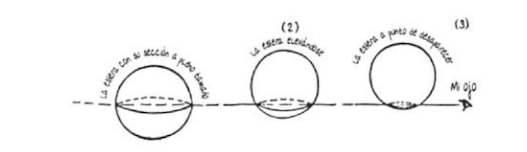
\includegraphics[width=0.6\textwidth]{esfera.png}
    }
    \caption{\textcolor{Victoria}{\textbf{Secciones de una esfera al atravesar el plano de Planilandia.}}}
    \label{fig:esfera-secciones}
\end{figure}

Aunque \textbf{Cuadrado} presencia todo esto con sus propios ojos, no logra comprender del todo lo que ocurre. El visitante, ahora identificado como una \textbf{Esfera}, intenta explicarlo mediante una analogía: un punto genera una línea, una línea genera un cuadrado, y un cuadrado, al moverse fuera del plano, genera un \underline{cubo}. De esta manera, la Esfera le sugiere que existen formas que van más allá de lo que su mundo puede imaginar.

Sin embargo, lejos de tranquilizar a \textbf{Cuadrado}, estas explicaciones lo alteran. La idea de un ser que existe fuera de su plano, en una dirección que no puede ver ni comprender, lo abruma por completo. El capítulo termina con \textbf{Cuadrado} perdiendo la paciencia y lanzándose contra la Esfera, sin entender todavía la verdadera naturaleza de lo que tiene frente a él.

\subsection*{Opinión personal}
\addcontentsline{toc}{subsection}{Opinión personal}

Este capítulo me pareció muy interesante porque muestra lo difícil que es entender algo cuando rompe por completo con lo que siempre hemos conocido. Aunque \textbf{Cuadrado} ve cómo la Esfera cambia de tamaño, su mente sigue atrapada en el plano. Me hizo pensar que muchas veces necesitamos más que solo pruebas para aceptar ideas que van más allá de nuestra forma habitual de pensar.

\section*{\textcolor{Horizon}{Capítulo 17: \emph{Cómo la Esfera, tras intentarlo en vano con las palabras, recurrió a los hechos}}}
\addcontentsline{toc}{section}{Capítulo 17: Cómo la Esfera, tras intentarlo en vano con las palabras, recurrió a los hechos}

\subsection*{Resumen}
\addcontentsline{toc}{subsection}{Resumen}

En este capítulo, \textbf{Cuadrado} intenta atacar a la \underline{\textbf{Esfera}} con toda su fuerza, esperando destruirla como a cualquier figura de Planilandia. Sin embargo, se da cuenta de que su embestida atraviesa al desconocido sin causarle daño, como si su cuerpo no perteneciera del todo a su mundo.

Al ver que con palabras no ha logrado convencerlo, la Esfera decide demostrar la verdad con \textbf{hechos}. Desde su posición fuera del plano, comienza a describir con total precisión lo que hay dentro de los muebles y habitaciones de la casa de \textbf{Cuadrado}, incluso objetos que están guardados y no pueden verse desde el plano. Cuando \textbf{Cuadrado} verifica que todo lo que dice es correcto, queda completamente \underline{impactado}.

La Esfera explica que puede ver el interior de todas las cosas porque se encuentra \emph{por encima del plano}, no dentro de él. También le ofrece a \textbf{Cuadrado} una prueba directa: toca su interior desde el espacio, provocándole un dolor súbito que no puede explicar de forma normal. Con esto, intenta hacerle entender que existe una realidad fuera del plano de Planilandia.

A pesar de todo esto, \textbf{Cuadrado} entra en pánico. Su seguridad comienza a romperse y, dominado por el miedo, intenta nuevamente atacar a la Esfera. Esta, al ver el peligro, decide actuar rápidamente y le anuncia que lo sacará de su plano para mostrarle la verdad de una vez por todas, quiera o no.

\subsection*{Opinión personal}
\addcontentsline{toc}{subsection}{Opinión personal}

Este capítulo me pareció muy intenso, porque la Esfera ya no solo explica, sino que demuestra lo que dice. Aun así, \textbf{Cuadrado} reacciona con miedo y violencia. Me hizo pensar que muchas veces, cuando algo rompe por completo nuestras creencias, en lugar de aceptarlo, primero tratamos de defendernos.


\section*{\textcolor{Cerulean}{Capítulo 18: \emph{Cómo fui a Espaciolandia y lo que vi allí}}}
\addcontentsline{toc}{section}{Capítulo 18: Cómo fui a Espaciolandia y lo que vi allí}

\subsection*{Resumen}
\addcontentsline{toc}{subsection}{Resumen}

En este capítulo, Cuadrado es llevado por la \textbf{Esfera} fuera de Planilandia hacia el mundo de las 
\textcolor{Apple Green}{\textbf{tres dimensiones}}, conocido como \emph{Espaciolandia}. Al inicio experimenta una sensación de terror y desorientación, pues su percepción ya no corresponde a nada conocido en su mundo bidimensional. Poco a poco, su guía le recomienda abrir los ojos y observar con atención.

Cuadrado logra ver por primera vez el \underline{interior real de las figuras}, comprendiendo que los seres de Espaciolandia no son simples círculos, sino cuerpos formados por infinitas secciones circulares: \textbf{esferas}. Entiende entonces que aquello que en Planilandia se ve como un círculo no es más que la \emph{proyección} de un sólido tridimensional.

\begin{figure}[H]
    \centering
    \fcolorbox{Cerulean}{pink}{
        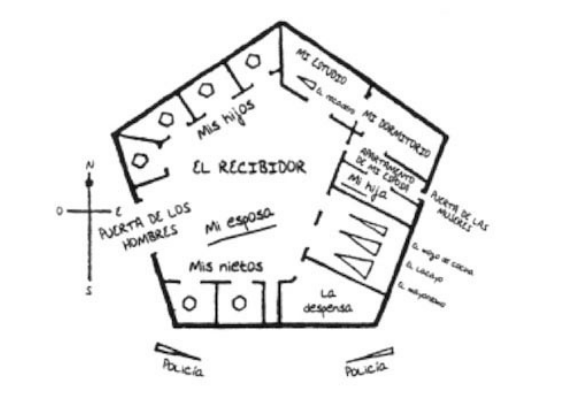
\includegraphics[width=0.65\textwidth]{espaciolandia.png}
    }
    \caption{\textcolor{Cerulean}{\textbf{Vista de Planilandia desde Espaciolandia. Representación tridimensional del espacio.}}}
    \label{fig:espaciolandia}
\end{figure}

Elevándose cada vez más, Cuadrado observa su ciudad natal desde arriba y queda impactado al mirar el interior de las casas, de su familia y hasta de los objetos. Todo lo que antes sólo podía suponer ahora lo ve con claridad. Más aún, llega a observar \underline{las minas, cavernas y estructuras internas del planeta}, lo que lo deja completamente asombrado.

Durante este viaje, la Esfera también reflexiona sobre el conocimiento y la omnisciencia, cuestionando si el hecho de poder verlo todo hace a los seres más justos o mejores. Finalmente, se dirigen hacia la \textbf{Gran Asamblea de Planilandia}, donde los gobernantes se reúnen para decidir el destino de aquellos que hablan de otros mundos.

Cuadrado reconoce a su propio hermano entre los miembros del consejo y se entera de que quienes han afirmado la existencia de otra dimensión han sido perseguidos y castigados severamente. En ese momento, la Esfera irrumpe ante los consejeros proclamando la existencia del país de las tres dimensiones, lo que provoca miedo, confusión y un inmediato intento de captura.

\subsection*{Opinión personal}
\addcontentsline{toc}{subsection}{Opinión personal}

Desde mi punto de vista, este capítulo es uno de los más fuertes hasta ahora, porque enfrenta directamente el conocimiento con el poder. La experiencia de Cuadrado en Espaciolandia resulta tan reveladora como inquietante.

Llama mucho la atención cómo, aun con pruebas claras, la Asamblea prefiere \underline{castigar antes que aceptar} una realidad que pone en riesgo su orden establecido. Esto hace que el capítulo se sienta muy actual.

Además, el contraste entre la inocente curiosidad de Cuadrado y la dureza del sistema que lo rodea refuerza la crítica del autor hacia las sociedades que temen cambiar.

\section*{\textcolor{Cerulean}{Capítulo 19: \emph{Cómo, aunque la esfera me mostró otros misterios de Espaciolandia, aún deseé conocer más; y lo que resultó de ello}}}
\addcontentsline{toc}{section}{Capítulo 19: Cómo, aunque la esfera me mostró otros misterios de Espaciolandia, aún deseé conocer más; y lo que resultó de ello}

\subsection*{Resumen}
\addcontentsline{toc}{subsection}{Resumen}

En este capítulo, Cuadrado intenta desesperadamente descender al consejo para interceder por su hermano, que está siendo llevado a prisión, pero descubre que ya no puede moverse por voluntad propia, pues depende completamente de la esfera. Ella le pide que no se preocupe por él y que continúe el viaje.

La esfera entonces le revela que hasta ahora solo le había mostrado \textbf{figuras planas}, pero que ha llegado el momento de conocer los \textbf{sólidos}. Para ello, comienza a apilar múltiples cuadrados uno sobre otro, no en dirección horizontal, sino \underline{uno encima del otro}, formando así un objeto completamente nuevo para Cuadrado: un \textbf{cubo}. 

Como se puede observar en la 
\textcolor{Lochmara}{\textbf{Figura \ref{fig:cubo_espaciolandia}}}, 
el cubo se construye mediante la superposición de planos iguales, lo cual permite entender cómo una figura de dos dimensiones puede dar origen a un sólido de tres dimensiones.

\begin{figure}[H]
    \centering
    \fcolorbox{Tarawera}{Tuscany}{
        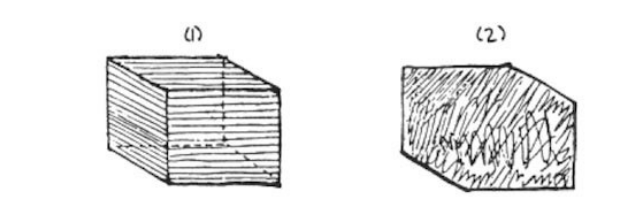
\includegraphics[width=0.65\textwidth]{cubo.png}
    }
    \caption{\textcolor{Tarawera}{\textbf{Construcción del cubo a partir de planos superpuestos, según la explicación de la esfera.}}}
    \label{fig:cubo_espaciolandia}
\end{figure}

Cuadrado, al ver el cubo, primero cree que se trata solo de una figura plana irregular, ya que no está acostumbrado a percibir la \textbf{profundidad}. La esfera le explica que su dificultad se debe a que nunca ha aprendido a interpretar la \emph{luz}, la \emph{sombra} y la \emph{perspectiva}, elementos esenciales para reconocer un sólido.

Gracias a las demostraciones de la esfera, Cuadrado logra finalmente comprender la diferencia entre un plano y un sólido, y reconoce que el cubo posee \textbf{seis caras} y \textbf{ocho vértices}. Esto lo llena de asombro, pues descubre que él mismo, como cuadrado en movimiento, es de cierta forma el origen de una figura tan compleja.

Sin embargo, su sed de conocimiento no se detiene ahí. Cuadrado desea comprender incluso el \underline{interior de la propia esfera}. Le pide que le muestre su contenido interno, pero la esfera se niega y le explica que no es posible hacerlo sin destruir su perfección. Aun así, Cuadrado insiste y comienza a hablar de la posible existencia de una \textbf{cuarta dimensión}, usando la misma lógica con la que antes se le reveló la tercera.

Entusiasmado por sus propias deducciones, Cuadrado imagina una sucesión infinita de dimensiones: cuarta, quinta, sexta, y aún más. Pero la esfera, molesta por esta ambición desmedida, lo interrumpe bruscamente. De pronto, Cuadrado es arrojado violentamente de regreso a Planilandia, cayendo en la oscuridad y despertando nuevamente en su estudio, como un simple cuadrado, escuchando la voz preocupada de su esposa.

\subsection*{Opinión personal}
\addcontentsline{toc}{subsection}{Opinión personal}

En este capítulo se siente con mucha fuerza el crecimiento interior de Cuadrado, pues ya no se conforma con aprender lo que se le muestra, sino que \textbf{quiere ir más allá por su cuenta}. Me gustó especialmente cómo, después de entender el cubo, su mente se lanza inmediatamente a imaginar nuevas dimensiones, mostrando un deseo de conocimiento que ya no puede detenerse.

También me pareció muy interesante la reacción de la esfera, porque refleja que incluso los maestros pueden tener límites y miedo ante lo desconocido. Este choque entre la curiosidad de Cuadrado y la negativa de la esfera deja una sensación de tensión que prepara el terreno para lo que sigue en la historia.


\section*{\textcolor{Tuscany}{Capítulo 20: \emph{Cómo me alentó la esfera en una visión}}}
\addcontentsline{toc}{section}{Capítulo 20: Cómo me alentó la esfera en una visión}

\subsection*{Resumen}
\addcontentsline{toc}{subsection}{Resumen}

Al inicio del capítulo, Cuadrado vuelve a su casa después de todas sus aventuras en Espaciolandia y decide \textbf{ocultar la verdad} a su esposa. Sabe que ella no podría comprender nada de lo que ha vivido, así que inventa una historia sencilla para tranquilizarla. Más tarde se retira a descansar, todavía con la mente llena de dudas sobre la tercera dimensión y sobre todo lo que ha visto.

Antes de quedarse dormido, Cuadrado se esfuerza por recordar la idea de \emph{“hacia arriba, pero no hacia el norte”}, que es la clave para imaginar la tercera dimensión. Poco a poco se duerme y entonces tiene un \textbf{sueño muy vívido}: vuelve a encontrarse con la Esfera, que ahora ya no está molesta con él, sino que parece más amable y luminosa. Ambos viajan a través del espacio hasta llegar a un pequeño punto brillante.

La Esfera le explica que ese lugar es \textcolor{Apple Green}{\textbf{Puntolandia}}, el reino donde sólo existe \textbf{una dimensión}, es decir, un simple punto sin largo, ancho ni altura. Allí vive un ser que se cree el centro de todo el universo y que no puede imaginar nada fuera de sí mismo. La Esfera invita a Cuadrado a observarlo con atención para que comprenda la lección que quiere enseñarle.

Cuadrado escucha al monarca de Puntolandia, quien habla de sí mismo como si fuera “todo en todo”. Para este ser, \underline{no existe nada más que él mismo}: no conoce otros puntos, ni líneas, ni figuras; sólo sabe de su propia existencia y se siente completamente feliz así. Al verlo, la Esfera le pide a Cuadrado que intente sacarlo de su \emph{autocomplacencia}, diciéndole algo parecido a lo que la propia Esfera le dijo a él cuando lo sacó de Planilandia.

Cuadrado entonces pronuncia un discurso para tratar de abrirle los ojos al rey de Puntolandia y mostrarle que su mundo es \textbf{muy limitado}. Sin embargo, el resultado es el contrario: el rey interpreta esas palabras como una confirmación de su grandeza y se siente todavía más orgulloso y satisfecho consigo mismo. Es decir, la explicación de Cuadrado no lo libera, sino que refuerza su egoísmo y su visión cerrada.

De regreso junto a la Esfera, Cuadrado se da cuenta de que sus palabras han servido de muy poco. La Esfera le explica que, cuando alguien está demasiado centrado en sí mismo, \textbf{ni siquiera una verdad más amplia logra cambiarlo}. Aun así, la Esfera anima a Cuadrado a seguir aspirando a dimensiones superiores, a no conformarse sólo con lo que conoce y a enseñar a otros a buscar siempre algo más allá de su propio mundo.

\subsection*{Opinión personal}
\addcontentsline{toc}{subsection}{Opinión personal}

Algo que me llamó la atención de este capítulo es el contraste entre Cuadrado y el rey de Puntolandia. Cuadrado acaba de descubrir un universo enorme, lleno de posibilidades, mientras que el rey es sólo un punto que no quiere saber nada más que de sí mismo. Me pareció una forma muy clara de mostrar cómo algunas personas se cierran tanto en su propia vida que ya no pueden ver nada fuera de ella.

También me gustó que la Esfera use esta visita como una especie de \emph{“clase extra”} para Cuadrado. No sólo le enseña geometría y dimensiones, sino que le muestra algo sobre la \textbf{actitud humana}: aspirar a más, querer comprender mejor el mundo, es mucho más valioso que quedarse cómodo en la ignorancia. Siento que el capítulo nos lanza una invitación suave pero fuerte a no conformarnos con lo que ya sabemos.

Por último, me pareció muy humana la figura de Cuadrado: quiere aprender más, quiere ir incluso a una cuarta dimensión, pero al mismo tiempo se equivoca, se emociona demasiado y sus palabras no siempre ayudan. Eso hace que el personaje se sienta cercano, como alguien que se esfuerza por crecer pero que todavía está aprendiendo a comunicar lo que ha descubierto.

\section*{\textcolor{vividviolet}{Capítulo 21: \emph{Cómo intenté enseñar la teoría de las tres dimensiones a mi nieto y con qué éxito}}}
\addcontentsline{toc}{section}{Capítulo 21: Cómo intenté enseñar la teoría de las tres dimensiones a mi nieto y con qué éxito}

\subsection*{Resumen}
\addcontentsline{toc}{subsection}{Resumen}

Al despertar lleno de entusiasmo, Cuadrado se siente llamado a difundir el \textbf{evangelio de las tres dimensiones} por toda Planilandia. Cree que ha descubierto una verdad tan grande que no puede guardársela sólo para sí mismo. Sin embargo, casi de inmediato escucha en la calle la proclamación del consejo, donde se ordena castigar con prisión o muerte a cualquiera que asegure haber recibido revelaciones de otros mundos. Esto lo obliga a actuar con extrema cautela.

Para no levantar sospechas, Cuadrado decide \textbf{ocultar la verdad a su esposa}, tranquilizándola con explicaciones vagas sobre lo ocurrido. Luego busca a alguien que pueda convertirse en su primer discípulo sin representar un peligro inmediato: su nieto, un joven hexágono aficionado a las matemáticas, a quien considera suficientemente inteligente y, al mismo tiempo, inocente frente a los asuntos del consejo.

A solas con él, retoman una lección de geometría elemental. Cuadrado le recuerda cómo un punto al moverse produce una línea, y cómo una línea en movimiento genera un cuadrado. A partir de ahí intenta dar el siguiente paso: explicarle que un cuadrado, al moverse \emph{“hacia arriba, pero no hacia el norte”}, puede producir una figura en tres dimensiones.

Justo entonces vuelve a oírse en la calle la voz del pregonero con la temida resolución del consejo. El nieto, al escuchar el anuncio, se llena de miedo y rompe en llanto. Asegura que nunca habló en serio de la tercera dimensión y que todo había sido un juego. Para él, la idea de moverse “hacia arriba” resulta absurda y peligrosa, algo propio de un disparate.

Cuadrado intenta salvar la situación tomando un cuadrado móvil y moviéndolo torpemente para mostrar lo que quiere decir con ese movimiento “hacia arriba”. Sin embargo, sus gestos no logran convencer al niño. El nieto termina riéndose, declara que su abuelo sólo estaba bromeando y sale corriendo de la habitación. De este modo, el primer intento de Cuadrado por enseñar la teoría de las tres dimensiones fracasa por completo.

\subsection*{Opinión personal}
\addcontentsline{toc}{subsection}{Opinión personal}

Desde mi punto de vista, este capítulo es uno de los más tristes y, al mismo tiempo, más realistas de toda la historia. Cuadrado está lleno de fe en lo que ha aprendido, pero se enfrenta de golpe con el miedo, la censura y la incomprensión, incluso dentro de su propia familia. Me dio la impresión de que la tercera dimensión, más que una revelación, se convierte aquí en una carga peligrosa que no puede compartirse libremente.

También me pareció muy significativa la reacción del nieto. No sólo muestra miedo, sino que además se ríe al final, como una forma inconsciente de protegerse de algo que no entiende. Esto me hizo pensar en cuántas veces, en la vida real, se ridiculiza lo desconocido simplemente porque resulta incómodo o amenaza lo que ya se considera seguro.

\section*{\textcolor{Tamarillo}{Capítulo 22: \emph{Cómo intenté luego difundir la teoría de las tres dimensiones por otros medios y del resultado}}}
\addcontentsline{toc}{section}{Capítulo 22: Cómo intenté luego difundir la teoría de las tres dimensiones por otros medios y del resultado}

\subsection*{Resumen}
\addcontentsline{toc}{subsection}{Resumen}

Después del fracaso con su nieto, Cuadrado no se rinde. Al contrario, comprende que no basta con una simple explicación verbal, así que decide intentar algo distinto: \textbf{escribir un libro}. En él quiere dejar constancia de todo lo que ha aprendido sobre las tres dimensiones, pero para evitar problemas con la ley, disfraza sus ideas hablando de un mundo imaginario llamado \emph{Pensamientolandia}, desde donde —en teoría— se podría observar el interior de todas las cosas.

Sin embargo, Cuadrado pronto se da cuenta de que su intento es casi inútil. En Planilandia no existen los diagramas reales, sólo líneas, por lo que su obra resulta difícil de entender para sus lectores. A pesar de haber terminado su tratado, siente que \underline{muy pocas personas lograrán comprender realmente lo que quiso decir}. Esto lo sumerge en una profunda tristeza y melancolía.

Con el paso del tiempo, su comportamiento se vuelve cada vez más extraño ante los demás. A veces, sin poder evitarlo, deja escapar comentarios sobre la tercera dimensión y sobre la posibilidad de ver el interior de las cosas. Poco a poco comienza a ser visto como un personaje peligroso, sospechoso de traición y de herejía.

Finalmente, en una reunión pública, Cuadrado ya no puede contenerse y \textbf{relata abiertamente toda su experiencia con la Esfera}. Aunque al principio intenta presentarlo como una historia ficticia, su pasión lo traiciona y termina afirmando la verdad con total convicción. El resultado es inmediato: es arrestado y llevado ante el Consejo.

Durante el juicio, Cuadrado se mantiene firme en su postura. No puede demostrar físicamente la tercera dimensión ni explicar con claridad qué significa \emph{“hacia arriba, no hacia el norte”}, pero insiste en la verdad de lo que vio. El Consejo decide no ejecutarlo, pero lo condena a \textbf{prisión perpetua} para evitar que sus ideas sigan propagándose.

Años después, Cuadrado sigue encerrado. Su propio hermano, a pesar de haber presenciado la llegada de la Esfera, aún no logra comprender la tercera dimensión. Cuadrado vive entre la esperanza y la duda: a veces cree firmemente en lo que vio, y otras veces teme que todo haya sido un sueño. Aun así, mantiene una última ilusión: que algún día, en otro mundo, alguien lea su historia y despierte a nuevas conciencias.

\subsection*{Opinión personal}
\addcontentsline{toc}{subsection}{Opinión personal}

Este capítulo me dejó una sensación muy fuerte de tristeza, porque Cuadrado intenta por todos los medios compartir la verdad y sólo recibe castigo a cambio. Su esfuerzo por escribir un libro y buscar nuevas formas de explicar lo que vio demuestra que realmente cree en su misión.

También me impactó que ni siquiera su propio hermano logre comprenderlo, a pesar de haber visto parte de los hechos. Esto muestra qué tan \textbf{profundamente cerrada} está la sociedad de Planilandia ante cualquier idea que rompa con lo establecido.

El final me pareció muy potente: Cuadrado queda solo, en prisión, con la duda de si todo fue real o no, pero con una última esperanza puesta en otros mundos. Siento que el autor nos deja una reflexión muy clara sobre lo difícil que es defender una verdad cuando va en contra de todo un sistema.







\end{document}
